\documentclass{article}
\PassOptionsToPackage{numbers,compress}{natbib}
\usepackage[preprint]{neurips_2025}
\usepackage[utf8]{inputenc}
\usepackage[T1]{fontenc}
\usepackage{hyperref}
\usepackage{url}
\usepackage{booktabs}
\usepackage{amsmath}
\usepackage{graphicx}
\usepackage{microtype}
\usepackage{amstext}

\title{Generating Paintings with a DCGAN on WikiArt}

\author{Ayushi Mishra \\ ECE 285, Homework 2 \\ \texttt{aymishra@ucsd.edu} \quad Code: \url{https://github.com/mishra37/ECE285-HW2}}

\begin{document}
\vspace{-2em}
\maketitle
\vspace{-1.5em}

\begin{abstract}
We train a DCGAN on the full WikiArt dataset (81{,}444 paintings, 27 styles) at $64\times64$ resolution. After 50 epochs it produces varied, painting-like images with recognizable compositions, palettes and brushstroke textures. FID (pool3 features, computed with PyTorch-Ignite) decreases steadily from 71.0 at epoch 10 to 22.0 at epoch 50. IS is $\approx3.0$.
\end{abstract}

\section{Method}
\paragraph{Data.} We use the WikiArt dataset from Kaggle (\texttt{steubk/wikiart}), all 27 style folders (81{,}444 images). We center-crop each image, resize it to $64\times64$ (bicubic) and cache all images once as a \texttt{uint8} array. For training, we scale pixels to $[-1,1]$ and flip images horizontally at random.

\paragraph{Model.} We follow DCGAN~\cite{radford2016dcgan}. The generator maps $z\sim\mathcal{N}(0,I_{100})$ through five transposed convolutions ($4\times4$, stride 2, channels $512\!\to\!256\!\to\!128\!\to\!64\!\to\!3$). Each layer uses BatchNorm and ReLU, and the last layer uses $\tanh$. The discriminator mirrors it with strided convolutions, BatchNorm and LeakyReLU(0.2), ending in a single logit. We initialize the weights from $\mathcal{N}(0,0.02)$. G has 3.6M and D 2.8M parameters.

\paragraph{Objective.} D minimizes binary cross-entropy on real vs.\ fake images. G uses the non-saturating loss $-\log D(G(z))$~\cite{goodfellow2014gan}. We apply one-sided label smoothing (real target 0.9)~\cite{salimans2016improved}.

\begin{table}[h]
\centering
\caption{Hyperparameters.}
\label{tab:hp}
\small
\begin{tabular}{ll@{\hspace{2em}}ll}
\toprule
Resolution & $64\times64\times3$ & Optimizer (G and D) & Adam, $\beta_1{=}0.5$, $\beta_2{=}0.999$ \\
Latent dim $n_z$ & 100 & Learning rate (G and D) & $2\times10^{-4}$ \\
Feature maps $n_{gf}, n_{df}$ & 64, 64 & Batch size & 128 \\
Real-label smoothing & 0.9 & Epochs / iterations & 50 / 31{,}800 \\
Augmentation & horizontal flip & Hardware & Kaggle, NVIDIA Tesla T4 \\
\bottomrule
\end{tabular}
\end{table}


\section{Results}
\begin{figure}[t]
\centering
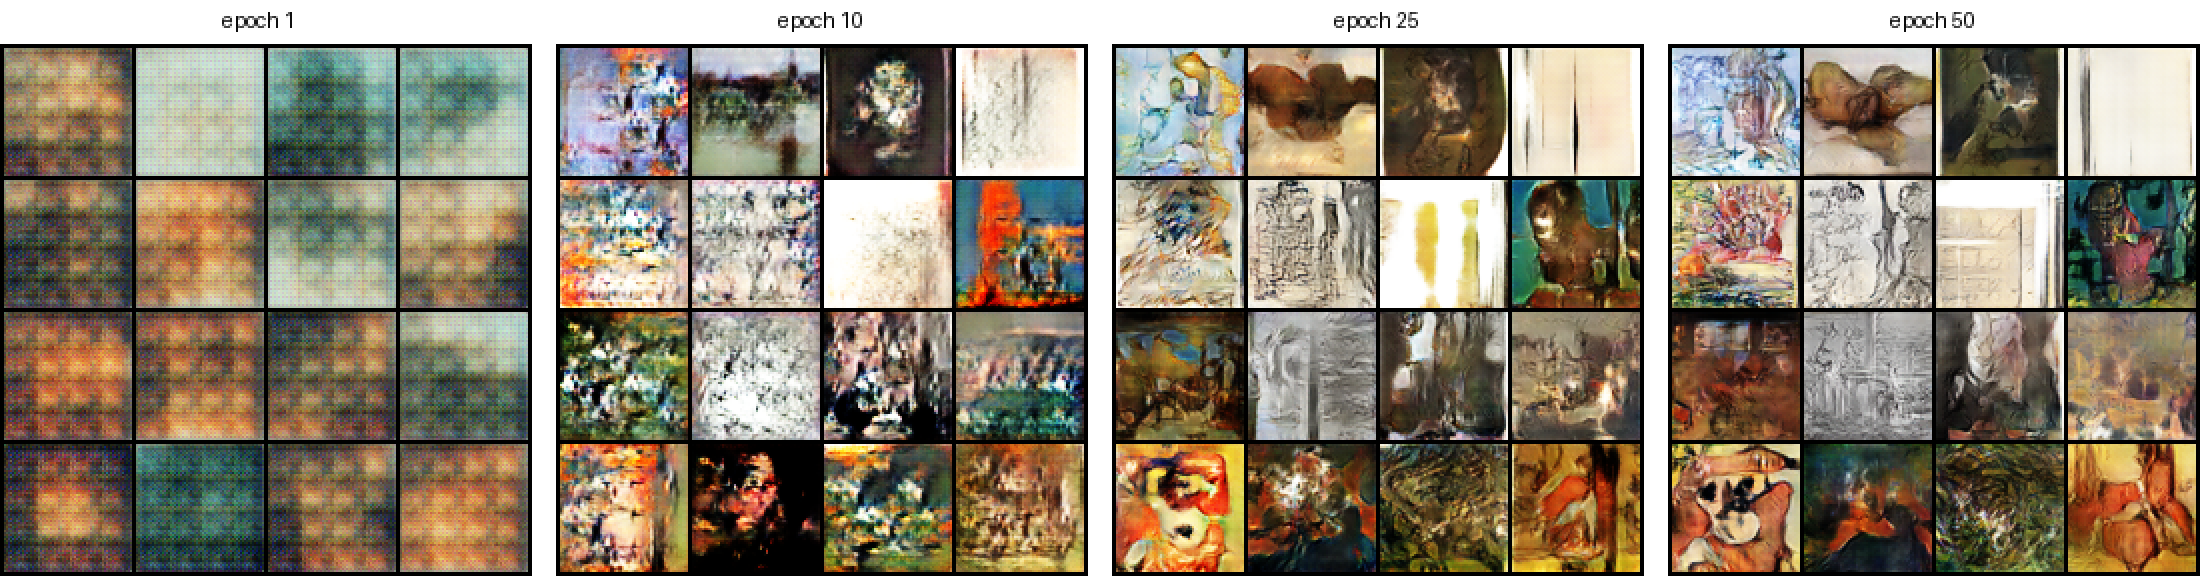
\includegraphics[width=0.94\linewidth]{figs/progression.png}\\[3pt]
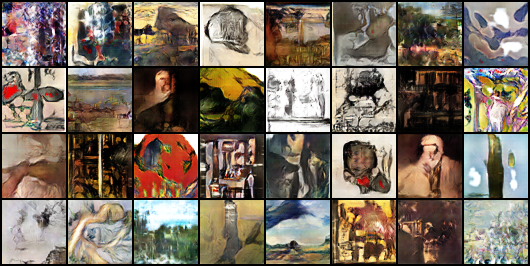
\includegraphics[width=0.46\linewidth]{figs/final_samples.png}\hspace{0.02\linewidth}
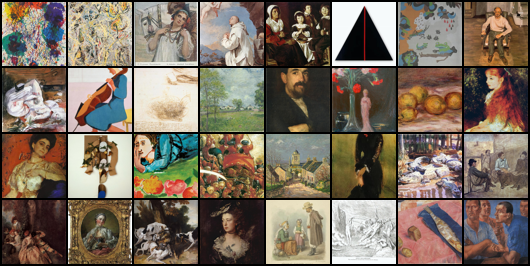
\includegraphics[width=0.46\linewidth]{figs/real.png}\vspace{-4pt}
\caption{Top: samples from the same fixed latent vectors at epochs 1, 10, 25 and 50. Bottom left: random samples from the final (epoch 50) generator. Bottom right: real WikiArt images at $64\times64$ for comparison.}
\label{fig:samples}
\end{figure}
\paragraph{Training dynamics.} Figure~\ref{fig:loss} shows the losses. At the start, the G loss spikes while D quickly learns to reject noise. After this short period, training is stable. The mean G loss falls from 5.2 at epoch 1 to $\approx$2.9 around epochs 18--30, with $D(x)\approx0.73$ and $D(G(z))\approx0.17$. Later, D slowly gains an edge (epoch 50: D loss 0.61, G loss 3.4, $D(G(z))=0.11$), and short loss spikes occur. Training always recovers, we see no mode collapse, and FID continues to decrease.

\begin{figure}[h]
\centering
\begin{minipage}[c]{0.6\linewidth}
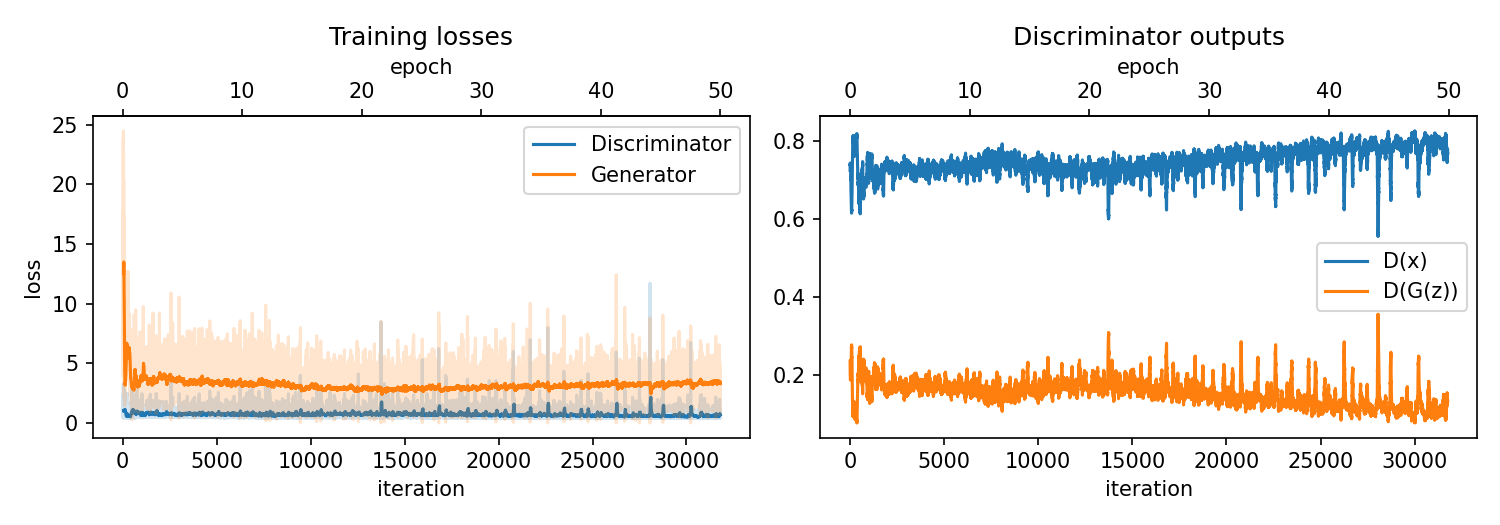
\includegraphics[width=\linewidth]{figs/loss_curves.png}
\end{minipage}\hfill
\begin{minipage}[c]{0.37\linewidth}
\centering\small
\begin{tabular}{lccc}
\toprule
Epoch & IS$\uparrow$ & FID$_\text{sm}\!\downarrow$ & FID$_\text{pool3}\!\downarrow$ \\
\midrule
10 & 2.31 & 0.068 & 71.0 \\
20 & 2.81 & 0.037 & 36.1 \\
30 & 3.04 & 0.037 & 30.1 \\
40 & 3.05 & 0.027 & 24.5 \\
50 & 3.02 & \textbf{0.022} & \textbf{22.0} \\
\bottomrule
\end{tabular}
\end{minipage}\vspace{-6pt}
\caption{Left: D and G losses per iteration (faint) and their 50-iteration moving average (solid). Middle: mean discriminator output on real ($D(x)$) and generated ($D(G(z))$) batches. Right: IS and FID on 10k generated vs.\ 10k real images. FID$_\text{sm}$ is Ignite's default (softmax features). FID$_\text{pool3}$ is the standard 2048-d version.}
\label{fig:loss}
\end{figure}

\paragraph{Quantitative evaluation.} We follow the provided PyTorch-Ignite tutorial. We take 10{,}000 generated and 10{,}000 random real images, map them to $[0,1]$, upsample them to $299\times299$ and give them to ImageNet Inception-v3. Ignite's default \texttt{FID()} compares 1000-d softmax outputs. Its values are much smaller than the standard FID~\cite{heusel2017fid}, so we also report FID on 2048-d pool3 features. Both FID variants decrease steadily during training (pool3 FID $71.0\to22.0$). This shows that sample quality continues to improve until epoch 50. IS increases from 2.3 to $\approx$3.0 and then stays level. IS is low in absolute terms because Inception-v3 learned from ImageNet photographs and rarely assigns confident classes to paintings. FID compares against real WikiArt images, so it is the more meaningful metric here.

\paragraph{Generated samples.} Figure~\ref{fig:samples} shows how samples evolve. At epoch 1, the generator only produces blurry colour blobs with checkerboard artifacts. At epoch 10, it produces painting-like palettes and canvas textures. At epochs 25--50, samples are sharper and show coherent compositions. Examples are landscapes, portrait-like figures on dark backgrounds, pencil sketches and abstract colour fields. Fine detail stays soft and figures and faces are often distorted. The $64\times64$ resolution is largely the cause.


\paragraph{Conclusion.}
A standard DCGAN learns the overall look of paintings (palettes, textures, coarse composition) from WikiArt. Training is stable over 50 epochs, and FID decreases from 71.0 to 22.0. Higher resolution, conditioning on style labels, or stronger architectures (spectral normalization, StyleGAN) would likely improve sharpness and FID further.

\vspace{-6pt}
{\footnotesize
\begin{thebibliography}{9}\setlength{\itemsep}{0pt}
\bibitem{goodfellow2014gan} I.~Goodfellow et al. Generative adversarial nets. \emph{NeurIPS}, 2014.
\bibitem{radford2016dcgan} A.~Radford et al. Unsupervised representation learning with deep convolutional GANs. \emph{ICLR}, 2016.
\bibitem{salimans2016improved} T.~Salimans et al. Improved techniques for training GANs. \emph{NeurIPS}, 2016.
\bibitem{heusel2017fid} M.~Heusel et al. GANs trained by a two time-scale update rule converge to a local Nash eq. \emph{NeurIPS}, 2017.
\end{thebibliography}}

\end{document}
